%\documentclass[jou]{apa6}
\documentclass[11pt]{article}
\usepackage{ucs}
\usepackage[utf8x]{inputenc}
\usepackage{changepage}
\usepackage{graphicx}
\usepackage{amsmath}
\usepackage{gensymb}
\usepackage{amssymb}
\usepackage{enumerate}
\usepackage{tabularx}
\usepackage{lipsum}
\usepackage{hyperref}
\usepackage{fancyvrb}

\oddsidemargin 0.0in
\evensidemargin 0.0in
\textwidth 6.27in
\headheight 1.0in
\topmargin -0.1in
\headheight 0.0in
\headsep 0.0in
\textheight 9.0in

\usepackage{xcolor}

\setlength{\parindent}{0pt}
\setlength{\columnsep}{1cm}

\newenvironment{myenv}{\begin{adjustwidth}{0.4in}{0.4in}}{\end{adjustwidth}}
\renewcommand{\abstractname}{Anotācija}
\renewcommand\refname{Atsauces}



\newcounter{alphnum}
\newenvironment{alphlist}{\begin{list}{(\Alph{alphnum})}{\usecounter{alphnum}\setlength{\leftmargin}{2.5em}} \rm}{\end{list}}


%16.3-6

\makeatletter
\let\saved@bibitem\@bibitem
\makeatother

\usepackage{bibentry}
%\usepackage{hyperref}


%\title{Homework 1: Grading Criteria}
%\author{Kalvis}
%\affiliation{RBS}



\begin{document}
\thispagestyle{empty}

\twocolumn


\begin{center}
{\Large Sample Assignment 1, 2020-09-09}
\end{center}



\vspace{10pt}
{\bf Question 1 (Memory Content).} Consider the following variable assignments:

\begin{center}
\begin{minipage}{.85\columnwidth}
\begin{Verbatim}[frame=single,numbers=left]
long long int a = -6;  
// Octal starts with "0"
long b = 0347;  
// TAB character
char c = '\t';  
\end{Verbatim}
\end{minipage}
\end{center}

Draw the memory content of these variables in {\em hexadecimal notation}. Ensure that the hex notation
length equals their actual length. You may need to add leading zeroes.

{\footnotesize
\begin{tabular}{|c|c|} \hline
{\bf Variable} & {\bf Hex value} \\ \hline
{\tt a} & \mbox{}\hspace{150pt}\mbox{} \\[10pt] \hline
{\tt b} & \\[10pt] \hline
{\tt c} & \\[10pt] \hline
\end{tabular}
}

\vspace{20pt}
{\bf Question 2 (Left and Right Shifts).} Write the output
(and the content of variables {\tt a,b,c} in hexadecimal notation),
after this snipped is executed:

\begin{center}
\begin{minipage}{.85\columnwidth}
\begin{Verbatim}[frame=single,numbers=left]
int a = 47;
int b = -13;
char c = 'c';
// bitwise AND
cout << (a & b) << endl;
// bitwise OR  
cout << (a | b) << endl;
// bitwise NOT
cout << (~b) << endl;
\end{Verbatim}
\end{minipage}
\end{center}

{\footnotesize
\begin{tabular}{|c|c|} \hline
{\bf Variable} & {\bf Hex value} \\ \hline
{\tt a} & \mbox{}\hspace{150pt}\mbox{} \\[10pt] \hline
{\tt b} & \\[10pt] \hline
{\tt c} & \\[10pt] \hline
Line 5 & \\[10pt] \hline
Line 7 & \\[10pt] \hline
Line 9 & \\[10pt] \hline
\end{tabular}
}




\vspace{20pt}
{\bf Question 3 (For-loops).}

Consider a regular "for" loop like this: 
\begin{verbatim}
for (int i=0; i<100; i++) { /*...*/ }
\end{verbatim}

\begin{enumerate}
\item Is it legal to change the loop variable {\tt i} 
in the body of the loop?
\item Is it legal to use the value {\tt i} after the loop 
has finished?
\item Can we omit the any of the three parts in the {\tt for}-loop?
Can we omit all $3$ parts as in this loop:\\ {\tt for (;;) { /* ... */ }}
\end{enumerate}



{\bf Question 4 (Flowchart to Code).} 
Write C++ code with branch and loop statements
(possibly, including "break" and "continue") to 
implement the flowchart shown in the picture.

\begin{center}
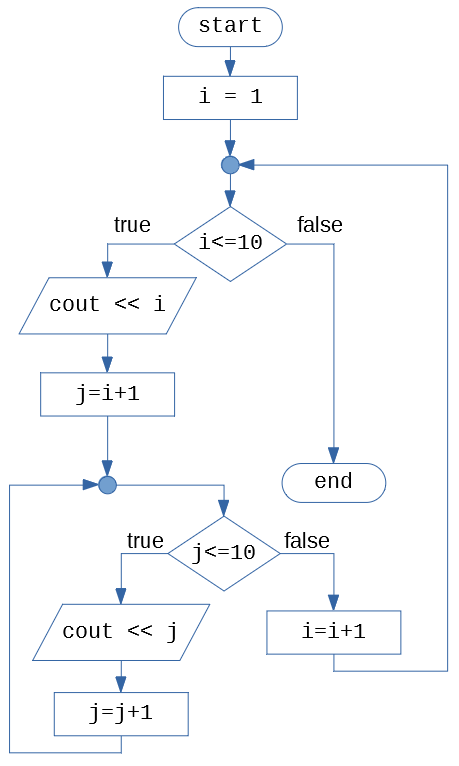
\includegraphics[width=2.7in]{assignment01-expr-control/assignment01-prob3-flowchart.png}
\end{center}



\vspace{20pt}
{\bf Question 5 (Code to Flowchart).}

For the code snippet below draw an equivalent flowchart. 
Does the "continue" statement jump to the bottom 
of the do-while loop (and retests the condition); 
or does it jump to the top of the do-while loop?
If you pass "null" user to the method {\tt isLast()} 
the program might crash.

{\footnotesize
\begin{center}
\begin{minipage}{.85\columnwidth}
\begin{Verbatim}[frame=single,numbers=left]
userDao.init();
do {    
  user = userDao.getNext();
  if (user == null) { continue; }
}
while (!user.isLast())
\end{Verbatim}
\end{minipage}
\end{center}
}

{\footnotesize
Please draw the flowchart nodes accurately: Use only $5$ kinds of nodes:\\
{\bf (1)} Start node (oval: one outgoing arrow).\\
{\bf (2)} Stop node (oval: one incoming arrow).\\
{\bf (3)} Conditional statement (diamond: one incoming and two outgoing arrows). Also mark the branch taken on {\tt true}. \\
{\bf (4)} Regular statement (rectangle: one incoming and one outgoing arrow).\\
{\bf (5)} Merging two branches (black dot: two incoming arrows, one outgoing arrow).
}

\newpage

{\bf \Large Solutions}

\vspace{10pt}
{\bf Question 1.} Answer:

\begin{tabular}{|c|r|} \hline
{\bf Variable} & {\bf Hex value} \\ \hline
{\tt a} & {\tt FFFFFFFFFFFFFFFA} \\ \hline
{\tt b} & {\tt 000000E7} \\ \hline
{\tt c} & {\tt 09} \\ \hline
\end{tabular}

To find {\tt a}, note that $-1$ has hex representation 
{\tt FFFFFFFFFFFFFFFF} ({\tt long long} is $8$ bytes long). 
To find $-6$, we subtract number $5$. Moreover, $\mathtt{F} - 5 = \mathtt{A}$ (in hex), 
since $15 - 5 - 10$ (in decimal).

To find {\tt b}, we transform from octal to hexadecimal through binary. 
Octal number $\mathtt{0347}_8$ is the 
same as $\mathtt{000.011.100.111}_2$.\\
Regroup the same bits (by four):\\
$\mathtt{0000.1110.0111}_2 = \mathtt{0E7}_{16}$. 
Type {\tt int} is $4$ bytes long.

To find {\tt c} look up the "TAB" character in the 
ASCII table \url{http://www.asciitable.com/}. 
It is the 9th byte that is written as {\tt 09}, since
{\tt char} is 1 byte long.

\vspace{20pt}
{\bf Question 2.} Answer:

\begin{tabular}{|c|r|} \hline
{\bf Variable} & {\bf Hex value} \\ \hline
{\tt a} & {\tt 0000002F} \\ \hline
{\tt b} & {\tt FFFFFFF3} \\ \hline
{\tt c} & {\tt 63} \\ \hline
Line 5 & $35$ \\ \hline
Line 7 & $-1$ \\ \hline
Line 9 & $12$ \\ \hline
\end{tabular}

{\footnotesize
\begin{verbatim}
a  = 0000.0000.0000.0000.0000.0000.0010.1111
b  = 1111.1111.1111.1111.1111.1111.1111.0011
============================================
L5 = 0000.0000.0000.0000.0000.0000.0010.0011
L7 = 1111.1111.1111.1111.1111.1111.1111.1111
L9 = 0000.0000.0000.0000.0000.0000.0000.1100
\end{verbatim}
}

In order to find the output for lines 5,7,9, we
can rewrite the hexadecimal content of {\tt a}, {\tt b}
as binary.\\
Line5 contains bit "1" 
in all those positions, where both {\tt a} AND {\tt b}
contains bit "1".\\
Line7 contains bit "1" where either {\tt a} OR {\tt b} 
contains bit "1".\\
Line9 contains bit "1" where {\tt b} contains bit "0" and vice versa.



\vspace{20pt}
{\bf Question 3.} Answer:

\begin{enumerate}
\item It is possible to change the loop variable inside {\tt for}
(this is certainly not recommended, because it violates usual 
intuition about the "for" loops). 
\item The value {\tt i} is usable after the body of loop, if
that variable is not declared inside the "for" loop statement itself,
but it is declared in a higher scope.
\item It is possible to omit any of the three parts in the "for" loop. 
If you skip all three, it is an infinite loop.
\end{enumerate}


\vspace{20pt}
{\bf Question 4.} Answer:

{\footnotesize
\begin{center}
\begin{minipage}{.85\columnwidth}
\begin{Verbatim}[frame=single,numbers=left]
int i, j;
for(i = 1; i <= 10; i = i+1) {
  cout << i; 
  for (j = i+1; j <= 10; j = j+1) {
    cout << j;
  }
}
\end{Verbatim}
\end{minipage}
\end{center}
}

The flowchart represents two nested "for" loops. 
Flowchart does not enforce "for" loops; it is possible 
to rewrite them as "while" loops as well.

{\footnotesize
\begin{center}
\begin{minipage}{.85\columnwidth}
\begin{Verbatim}[frame=single,numbers=left]
int i, j;
i = 1; 
while (i <= 10) {
  cout << i; 
  j = i+1;
  while (j <= 10) {
    cout << j;
    j = j+1;
  }
  i = i+1;
}
\end{Verbatim}
\end{minipage}
\end{center}
}


\vspace{20pt}
{\bf Question 5.} Answer:


\begin{center}
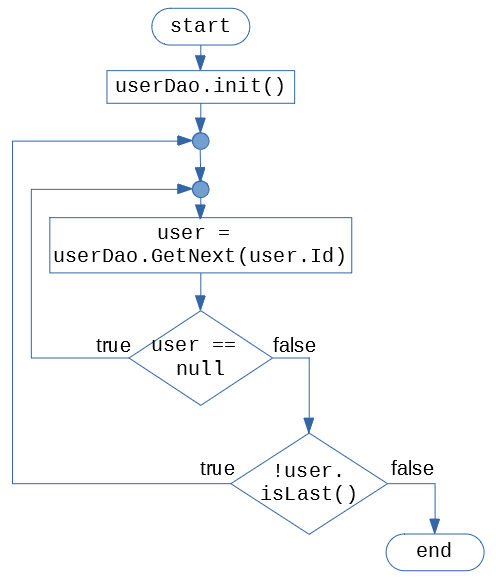
\includegraphics[width=2.7in]{assignment01-expr-control/assignment01-prob5-flowchart.png}
\end{center}


\end{document}



